\chapter{PENGUJIAN DAN ANALISIS}
\label{chap:pengujiananalisis}

% Ubah bagian-bagian berikut dengan isi dari pengujian dan analisis

Pada penelitian ini dilakukan uji dan analisis dari model prediksi yang sudah dibuat. Pengujian ini dilakukan dengan beberapa skenario pengujian. Dalam pengujian ini akan diambil data yang akan merujuk pada performa sistem yang telah dibuat. Data - data yang diambil juga akan divisualisasikan untuk mendapatkan indikasi terkait hasil tugas akhir yang telah dilakukan.

\section{Pengujian}
\label{sec:skenariopengujian}

Pada subbab ini dilakukan beberapa skenario pengujian terhadap model untuk mengetahui performa dan tingkat kesalahan yang dapat membuka kesempatan pengembangan penelitian di masa depan serta menarik kesimpulan secara keseluruhan. Berikut adalah skenario pengujian yang dilakukan.

\subsection{Hasil Pengujian Performa menggunakan YOLOV8}
Dalam pembuatan model yang digunakan, dilakukan pengambilan dan labeling data citra yang akan digunakan sebagai set data pelatihan atau set data \emph{train}. Dimana data yang digunakan pada sistem yang akan dibuat menggunakan data citra manusia yang telah dijabarkan pada bab sebelumnya.

Data yang digunakan sebagai set data berjumlah  1735 data citra manusia. Dalam pengembangan model nantinya data citra ini akan dibagi menjadi 2 bagian dimana sebesar 1435 data citra sebagai set pelatihan dan sisanya sebesar 300 data citra akan digunakan sebagai set validasi. Setelah proporsi dataset ditentukan maka API key akan digenerate pada roboflow yang nantinya akan dipanggil untuk dilakukan proses training. 

Setelah proses pemuatan set dilakukan, maka akan dilajutkan pada proses training model. Proses training dilakukan dengan menggunakan beberapa parameter, yang dimana parameter ini akan dibandingkan performanya melalui nilai confusion matrix maupun nilai akurasi deteksi seperti presisi , recall, mapupun classification loss.

Pelatihan pertama menggunakan 100\emph{epoch} dan \emph{batch size} sebesar 16 dengan tindakan praproses merubah ukuran gambar pada dataset menjadi 800x800 piksel dengan pemberian augmentasi berupa 90\textdegree rotasi dan noise. Penggunaan augmentasi ini menambah jumlah data citra yang semulanya 1435 menjadi 4305. Adapun tujuan dari pelatihan ini untuk mengetahui seberapa baik peningkatan model pre- trained yang digunakan dalam deteksi manusia dengan menggunakan dataset yang teraugmentasi.

Didapatkan nilai box loss pada proses training menggunakan YOLOV8 ini adalah sebesar 0.819 setelah 100 epoch. Box loss mengukur seberapa baik model memprediksi bounding boxes seputar objek. Loss ini umumnya dihitung menggunakan metode seperti Intersection over Union (IoU) atau variasinya seperti CIoU atau DIoU, yang mengukur kesesuaian antara bounding box yang diprediksi dengan ground truth. Tujuan dari loss ini adalah untuk mengoptimalkan model agar bounding box yang diprediksi sesuai dengan posisi dan ukuran objek sebenarnya dalam gambar. Adapun penurunan yang nilai box loss yang didapatkan selama training menandakan bahwa hasil training yang dilakukan telah berhasil membuat model menentukan koordinat bounding box pada object manusia dengan akurat.

Didapatkan nilai box loss pada proses validasi menggunakan YOLOV8 ini sebesar 1.2 , adapun box loss pada validasi ini mengindikasikan kemampuan mengenali objek pada data uji. Secara teori, penurunan object loss pada tahap validasi menandakan bahwa model mampu melakukan deteksi objek secara umum. bukan hanya pada data pelatihan.

Skor mAP pada threshold 0.5 yang diperoleh pada proses ini adalah sebesar 80.9\% dimana nilai ini mengindikasikan bahwa model memiliki kemampuan yang baik untuk mendeteksi objek dengan ketepatan yang tinggi, dengan syarat kriteria IoU minimal 0.5 terpenuhi. Ini mengindikasikan dalam banyak percobaan kasus, bounding box yang diprediksi oleh model memiliki overlap yang signifikan dengan bounding box ground truth.

Nilai nilai yang dicantumkan juga dapat dilihat lebih detail pada visualiasi berikut ini. Dimana nilai visualisasi cenderung turun pada Box loss dan cenderung naik pada skor mAP. 

\begin{figure}[H]
    \centering
    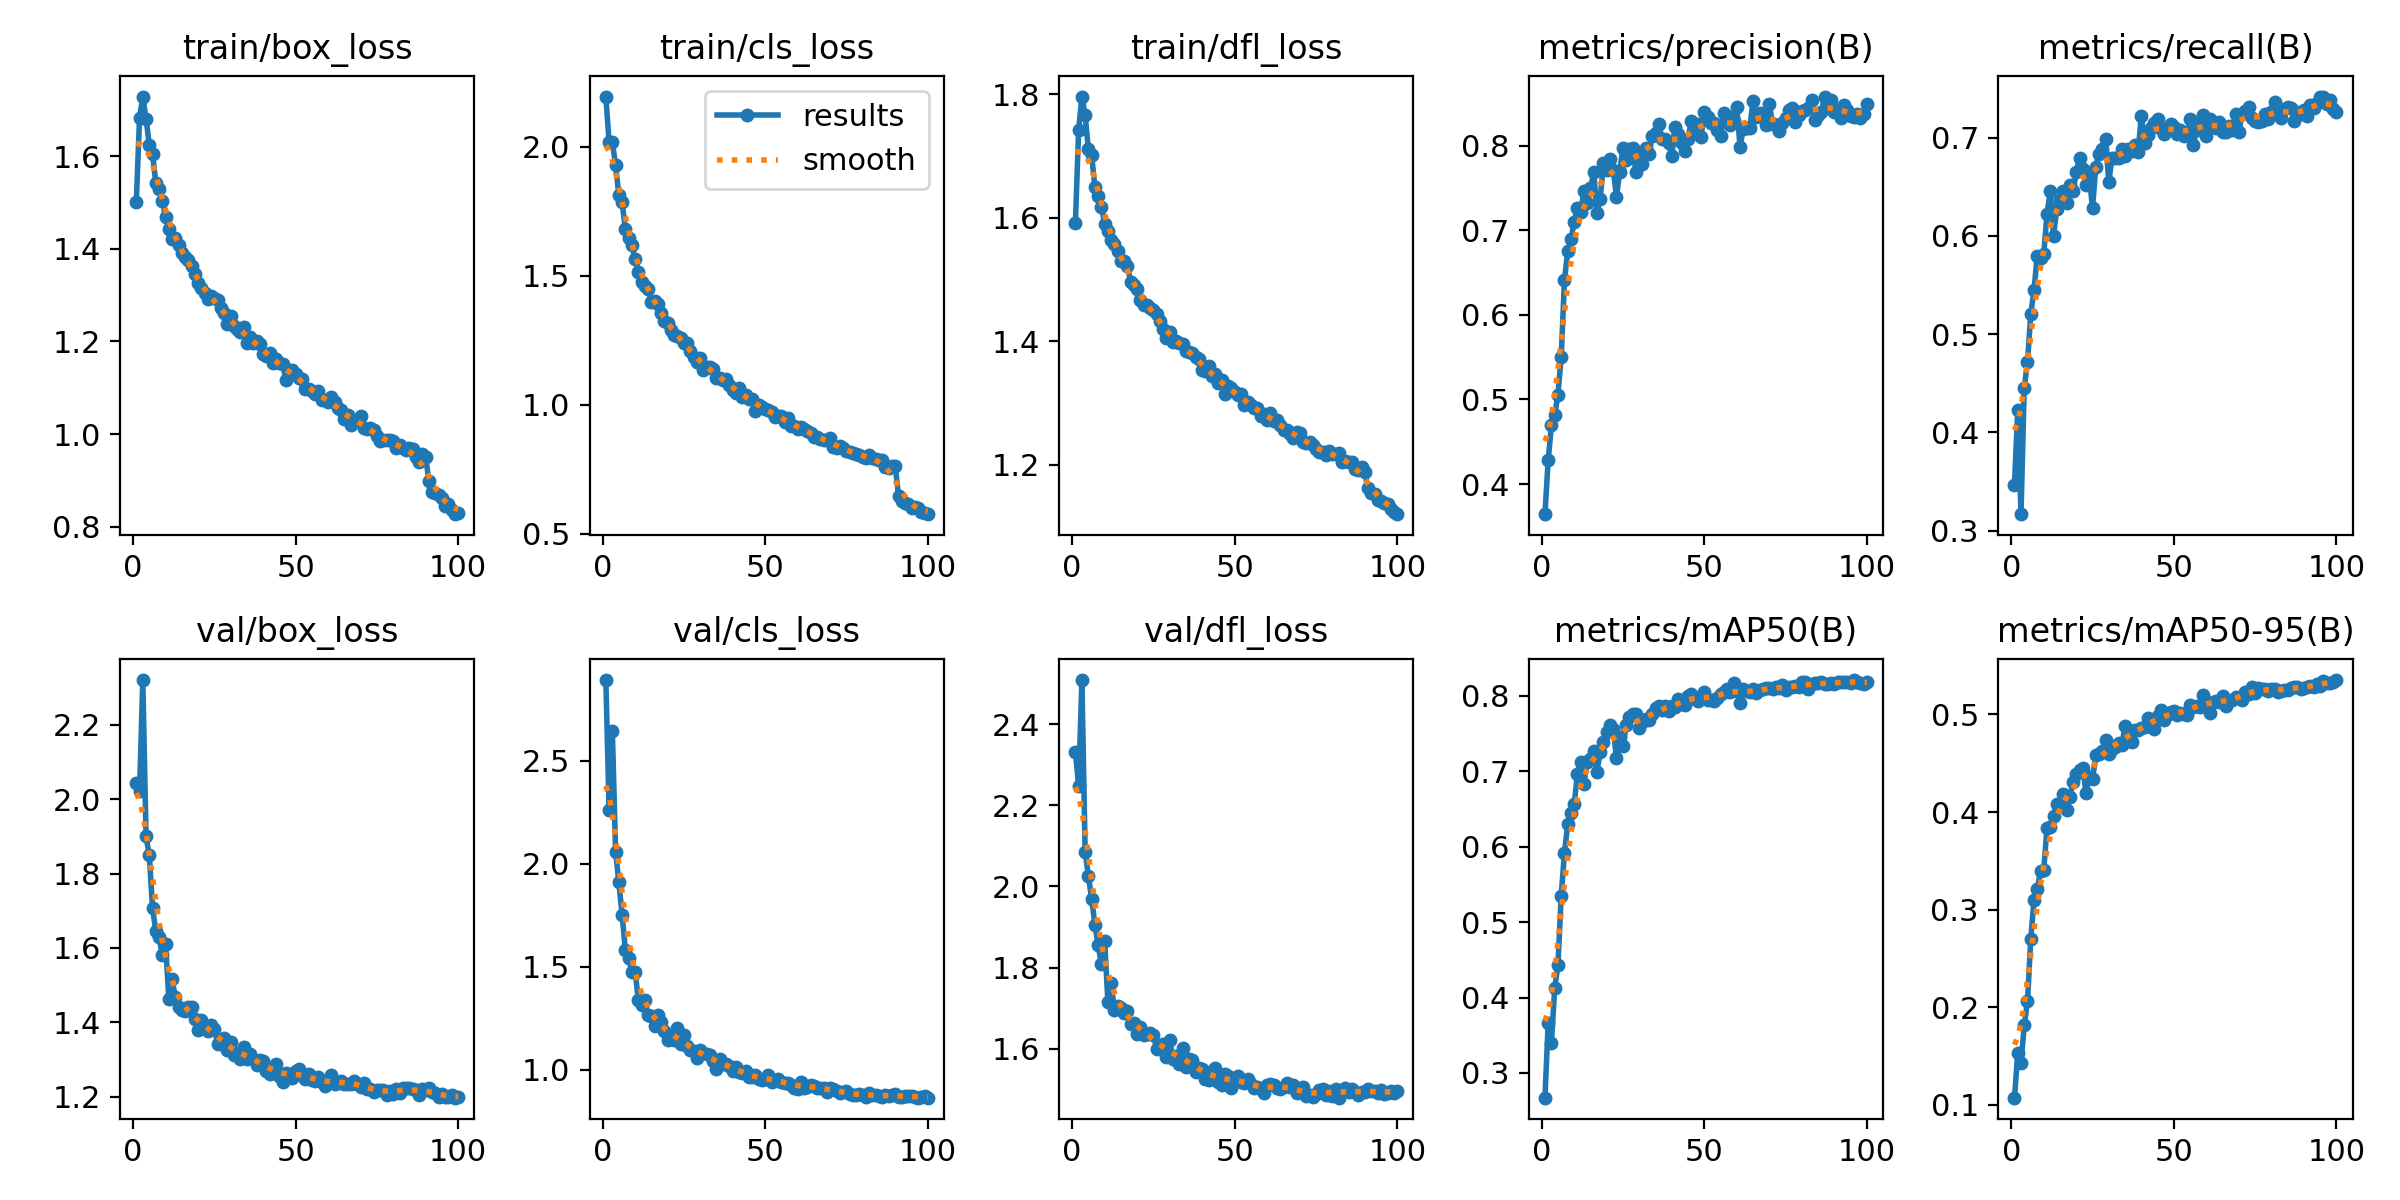
\includegraphics[scale=0.4]{gambar/loss 100 epoch.png}
    \caption{Visualisasi Hasil training}
    \label{fig:visualisasi hasil training}
\end{figure}

Adapun visualisasi melalui confusion matrix yang digunakan, untuk merepresentasikan hasil model lebih detail. Adapun indikator pada confusion matrix pada setiap kotaknya merepresentasikan nilai \emph{true positive}, \emph{false positive}, \emph{false negative}, \emph{true negative} sesuai dengan bahasan pada bab sebelumnya dapat dilihat pada gambar berikut ini. 

\begin{figure}[H]
    \centering
    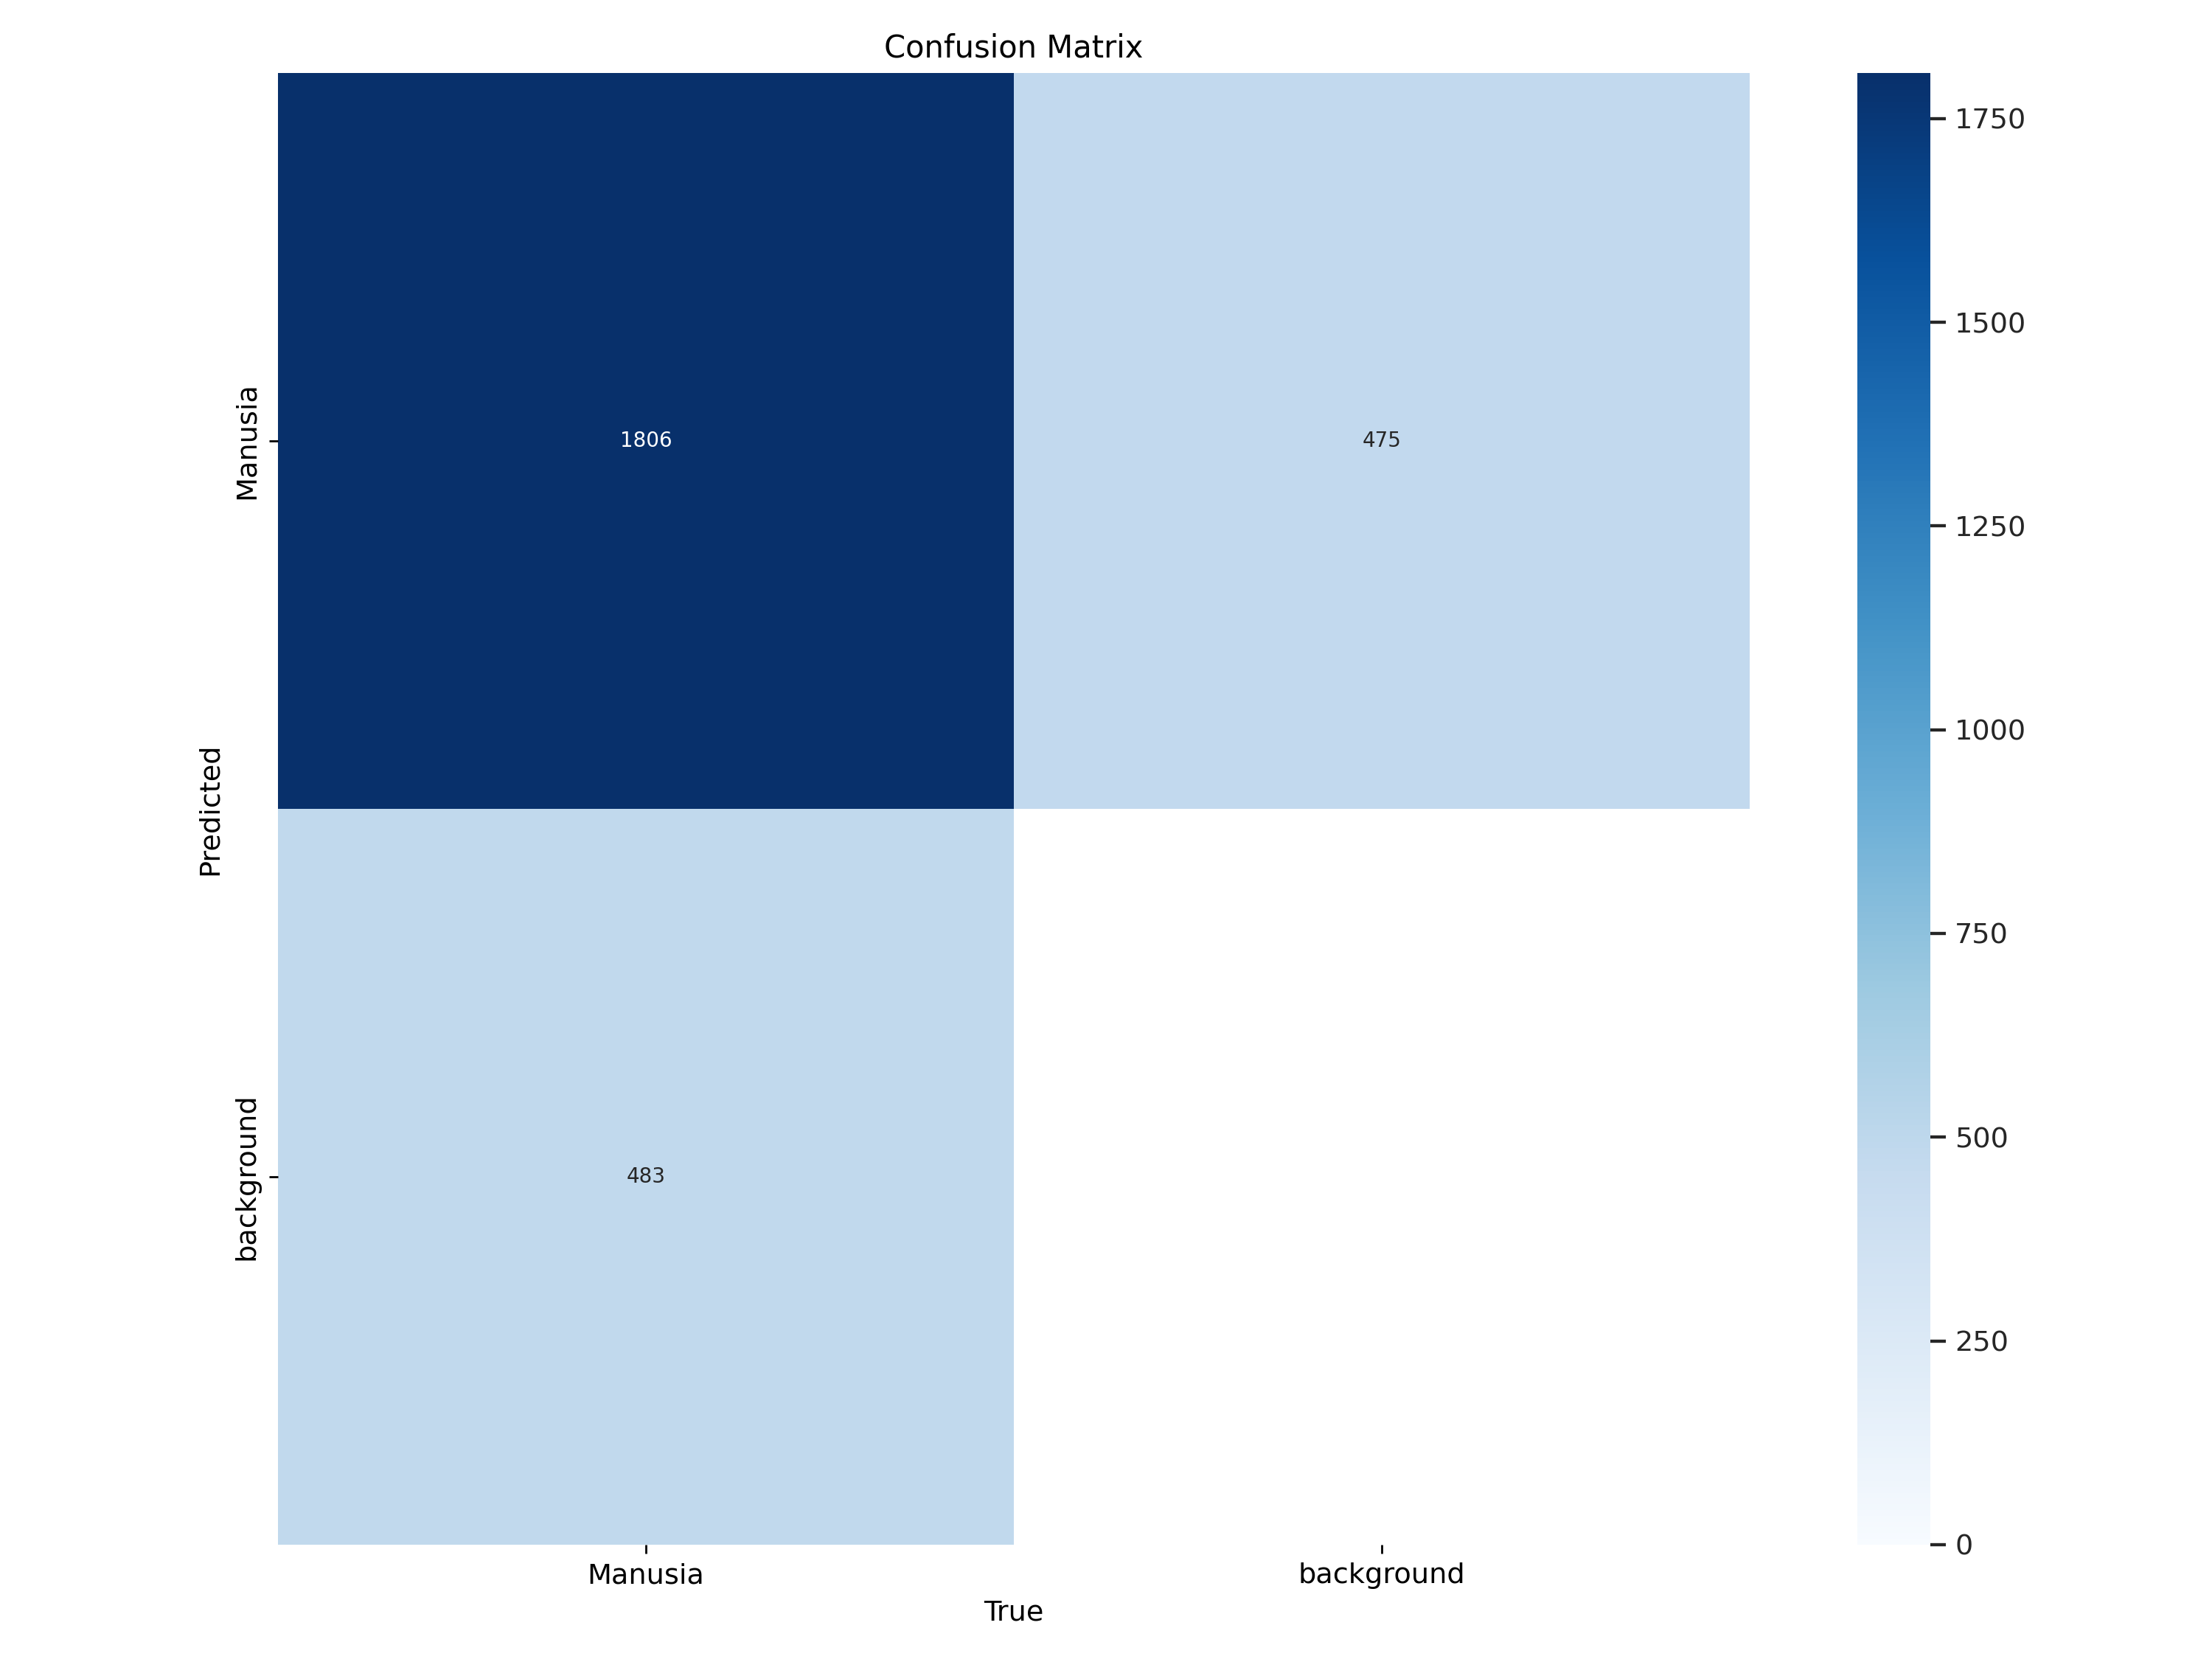
\includegraphics[scale=0.4]{gambar/confusion 100epoch.png}
    \caption{Confusion Matrix Hasil Training}
    \label{fig:visualisasi hasil training}
\end{figure}

Dapat dilihat pada dapat dilihat bahwa dari hasil klasifikasi model terdapat 1806 data citra yang termasuk dalam kategori true positive, 475 citra yang termasuk dalam kategori false positive dan 483 citra yang termasuk false negative.

Dilakukan pula tes inference model yang telah dilatih menggunakan set data test terhadap object manusia. Dapat dilihat pada gambar dibawah nilai confidence score yang cukup tinggi.

\begin{figure}[H]
    \centering
    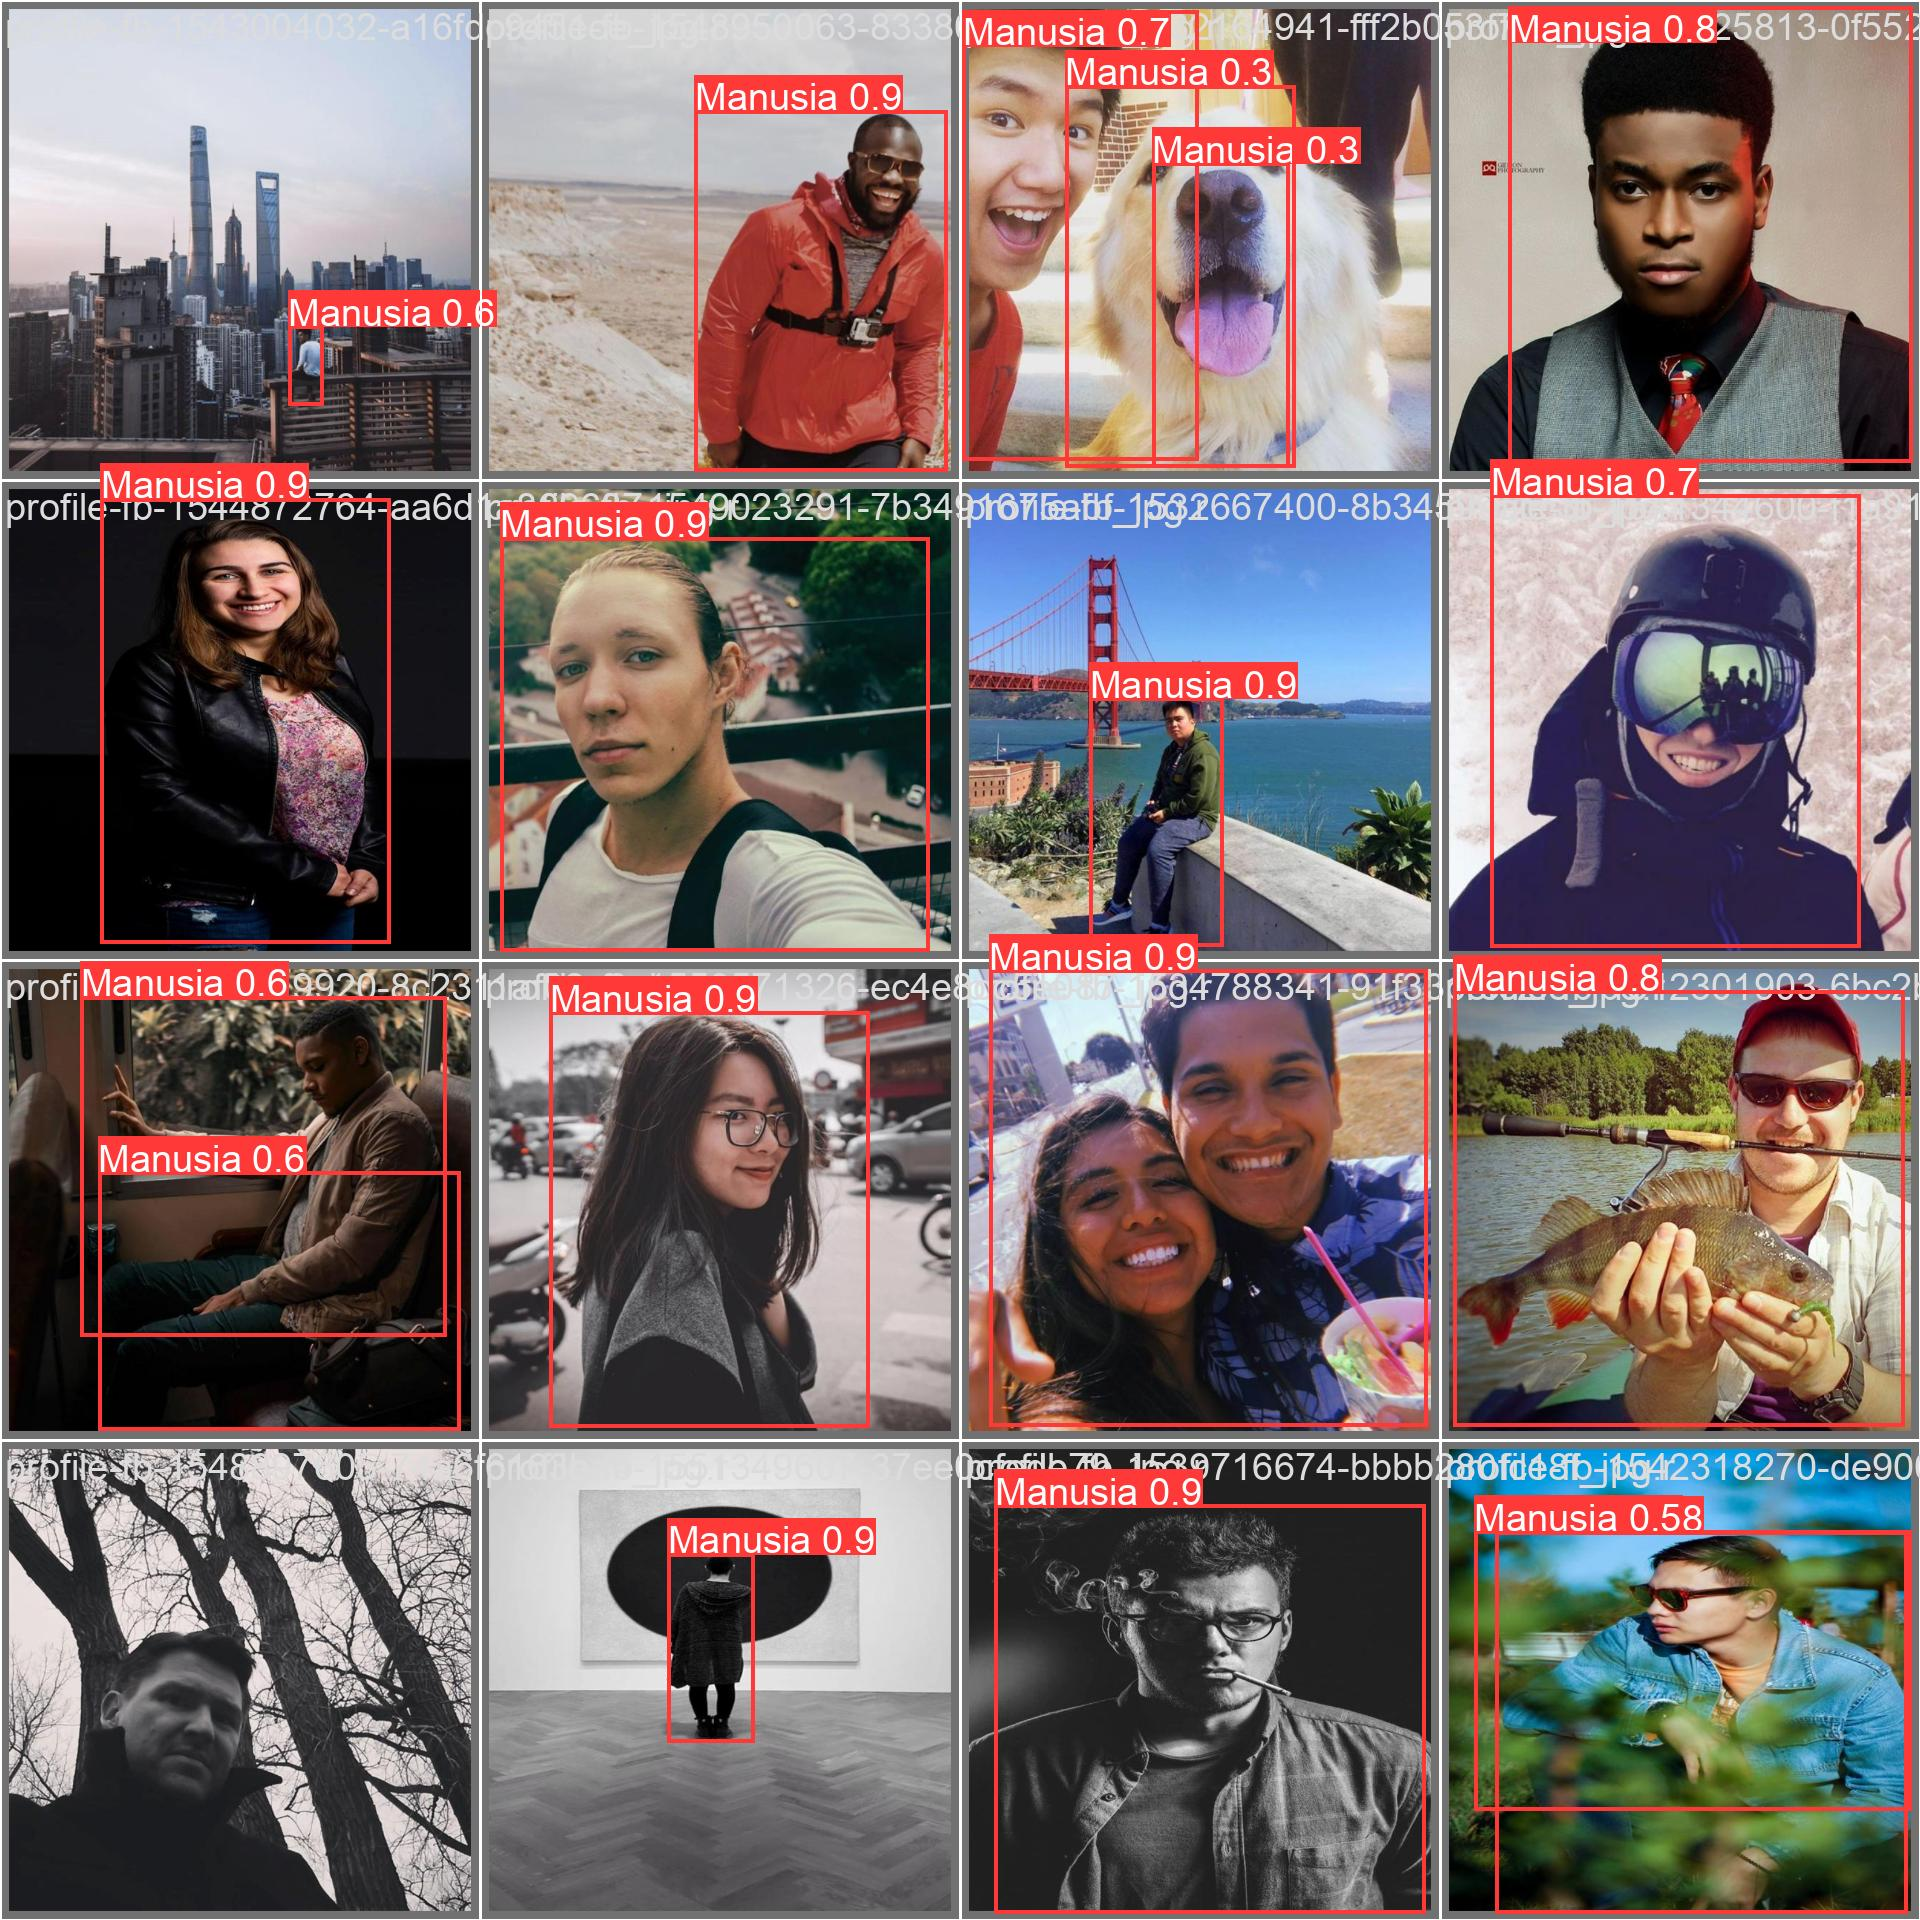
\includegraphics[scale=0.1]{gambar/confiden 100 epoch.jpg}
    \caption{Tes Inferensi Menggunakan Model Terlatih}
    \label{fig:visualisasi hasil training}
\end{figure}

\begin{figure}[H]
    \centering
    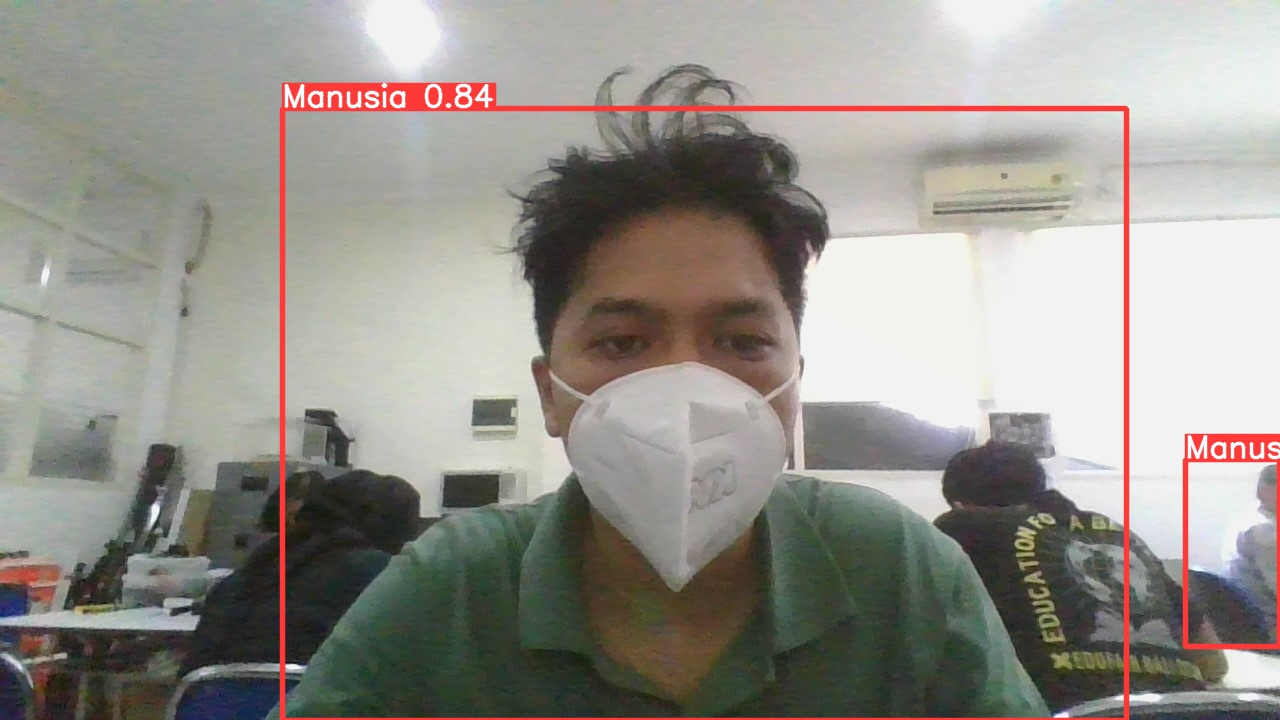
\includegraphics[scale=0.2]{gambar/confiden foto agung 100 epoch.jpg}
    \caption{Tes Inferensi Menggunakan Model Terlatih}
    \label{fig:enter-label}
\end{figure}

Pelatihan kedua menggunakan 150 \emph{epoch} dan \emph{batch size} sebesar 16 dengan tindakan pra proses merubah ukuran gambar pada dataset menjadi 800x800 piksel dengan pemberian augmentasi berupa 90\textdegree rotasi dan noise. Adapun tujuan dari pelatihan ini untuk mengetahui seberapa baik peningkatan model pre- trained yang digunakan dalam deteksi manusia dengan menggunakan dataset yang teraugmentasi.

Didapatkan nilai box loss pada proses training menggunakan YOLOV8 ini adalah sebesar 0.7383 setelah 150 epoch. Box loss mengukur seberapa baik model memprediksi bounding boxes seputar objek. Loss ini umumnya dihitung menggunakan metode seperti Intersection over Union (IoU) atau variasinya seperti CIoU atau DIoU, yang mengukur kesesuaian antara bounding box yang diprediksi dengan ground truth. Tujuan dari loss ini adalah untuk mengoptimalkan model agar bounding box yang diprediksi sesuai dengan posisi dan ukuran objek sebenarnya dalam gambar. Adapun penurunan yang nilai box loss yang didapatkan selama training menandakan bahwa hasil training yang dilakukan telah berhasil membuat model menentukan koordinat bounding box pada object manusia dengan akurat.

Didapatkan nilai box loss pada proses validasi menggunakan YOLOV8 ini sebesar 1.2143, adapun box loss pada validasi ini mengindikasikan kemampuan mengenali objek pada data uji. Secara teori, penurunan object loss pada tahap validasi menandakan bahwa model mampu melakukan deteksi objek secara umum. bukan hanya pada data pelatihan.

Skor mAP pada threshold 0.5 yang diperoleh pada proses ini adalah sebesar 81,7\% dimana nilai ini mengindikasikan bahwa model memiliki kemampuan yang baik untuk mendeteksi objek dengan ketepatan yang tinggi, dengan syarat kriteria IoU minimal 0.5 terpenuhi. Ini mengindikasikan dalam banyak percobaan kasus, bounding box yang diprediksi oleh model memiliki overlap yang signifikan dengan bounding box ground truth.

Nilai nilai yang dicantumkan juga dapat dilihat lebih detail pada visualiasi berikut ini. Dimana nilai visualisasi cenderung turun pada Box loss dan cenderung naik pada skor mAP. 

\begin{figure}[H]
    \centering
    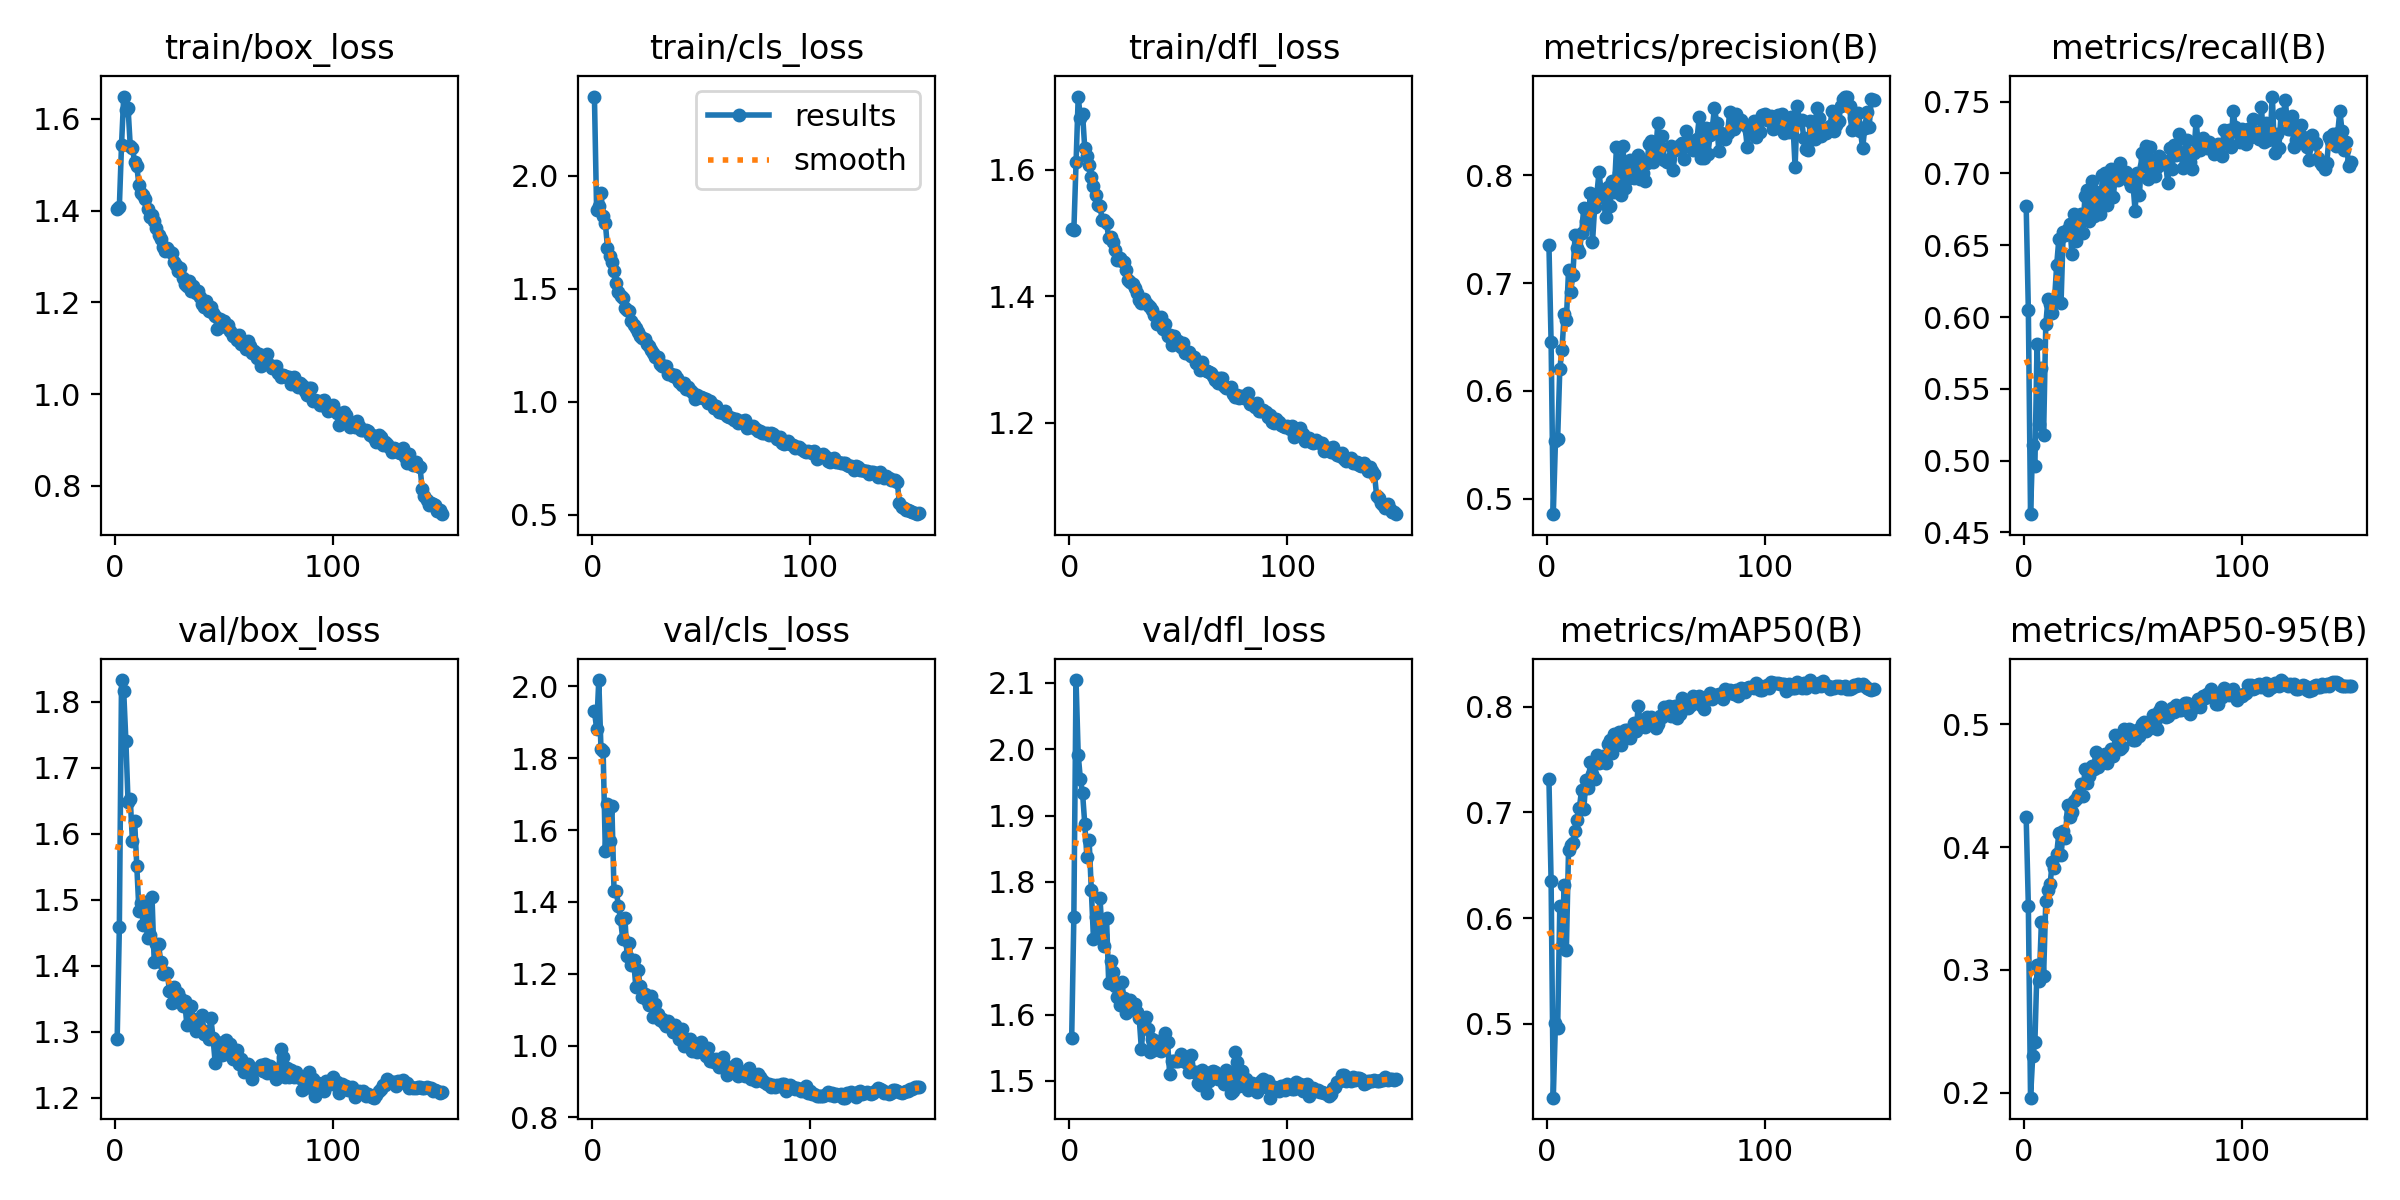
\includegraphics[scale=0.4]{gambar/loss 150 epoch.png}
    \caption{Visualisasi Hasil training}
    \label{fig:visualisasi hasil training}
\end{figure}


\begin{figure}[H]
    \centering
    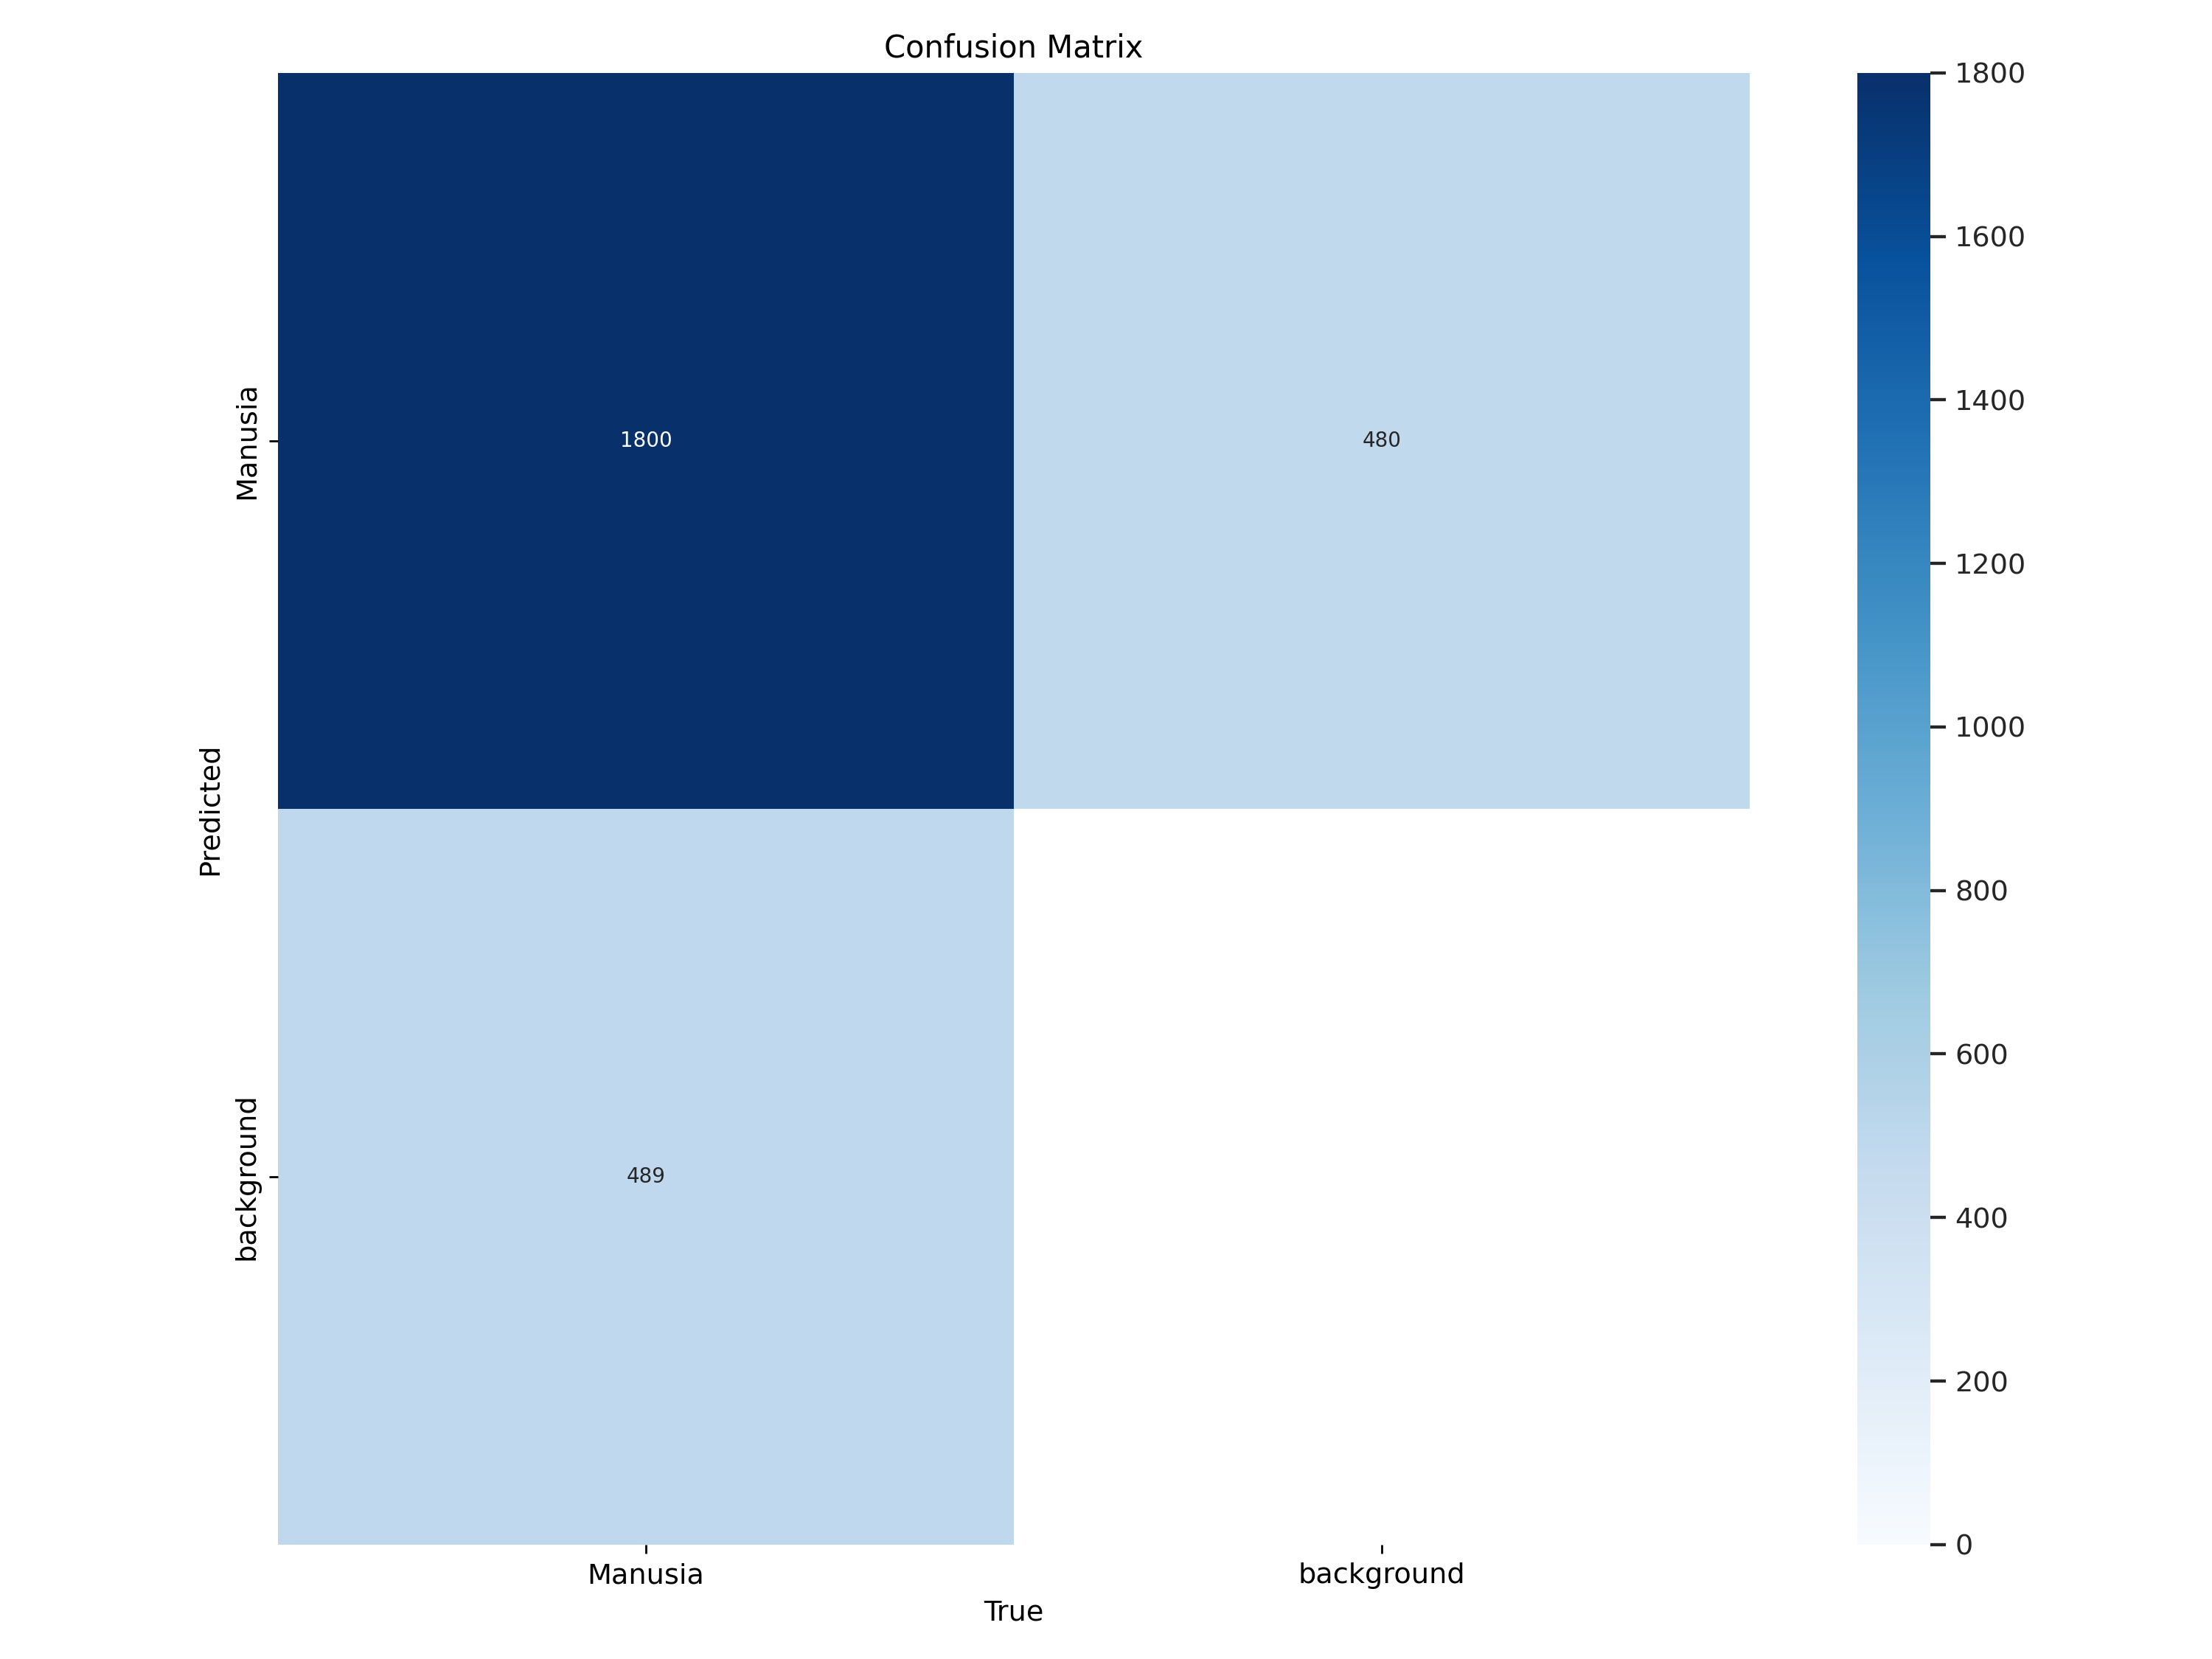
\includegraphics[scale=0.4]{gambar/confusion 150 epoch.png}
    \caption{Confusion Matrix Hasil Training}
    \label{fig:visualisasi hasil training}
\end{figure}

Dapat dilihat pada dapat dilihat bahwa dari hasil klasifikasi model terdapat 1800 data citra yang termasuk dalam kategori true positive, 480 citra yang termasuk dalam kategori false positive dan 489 citra yang termasuk false negative.

Dilakukan pula tes inference model yang telah dilatih menggunakan set data test terhadap object manusia. Dapat dilihat pada gambar dibawah nilai confidence score yang cukup tinggi.

\begin{figure}[H]
    \centering
    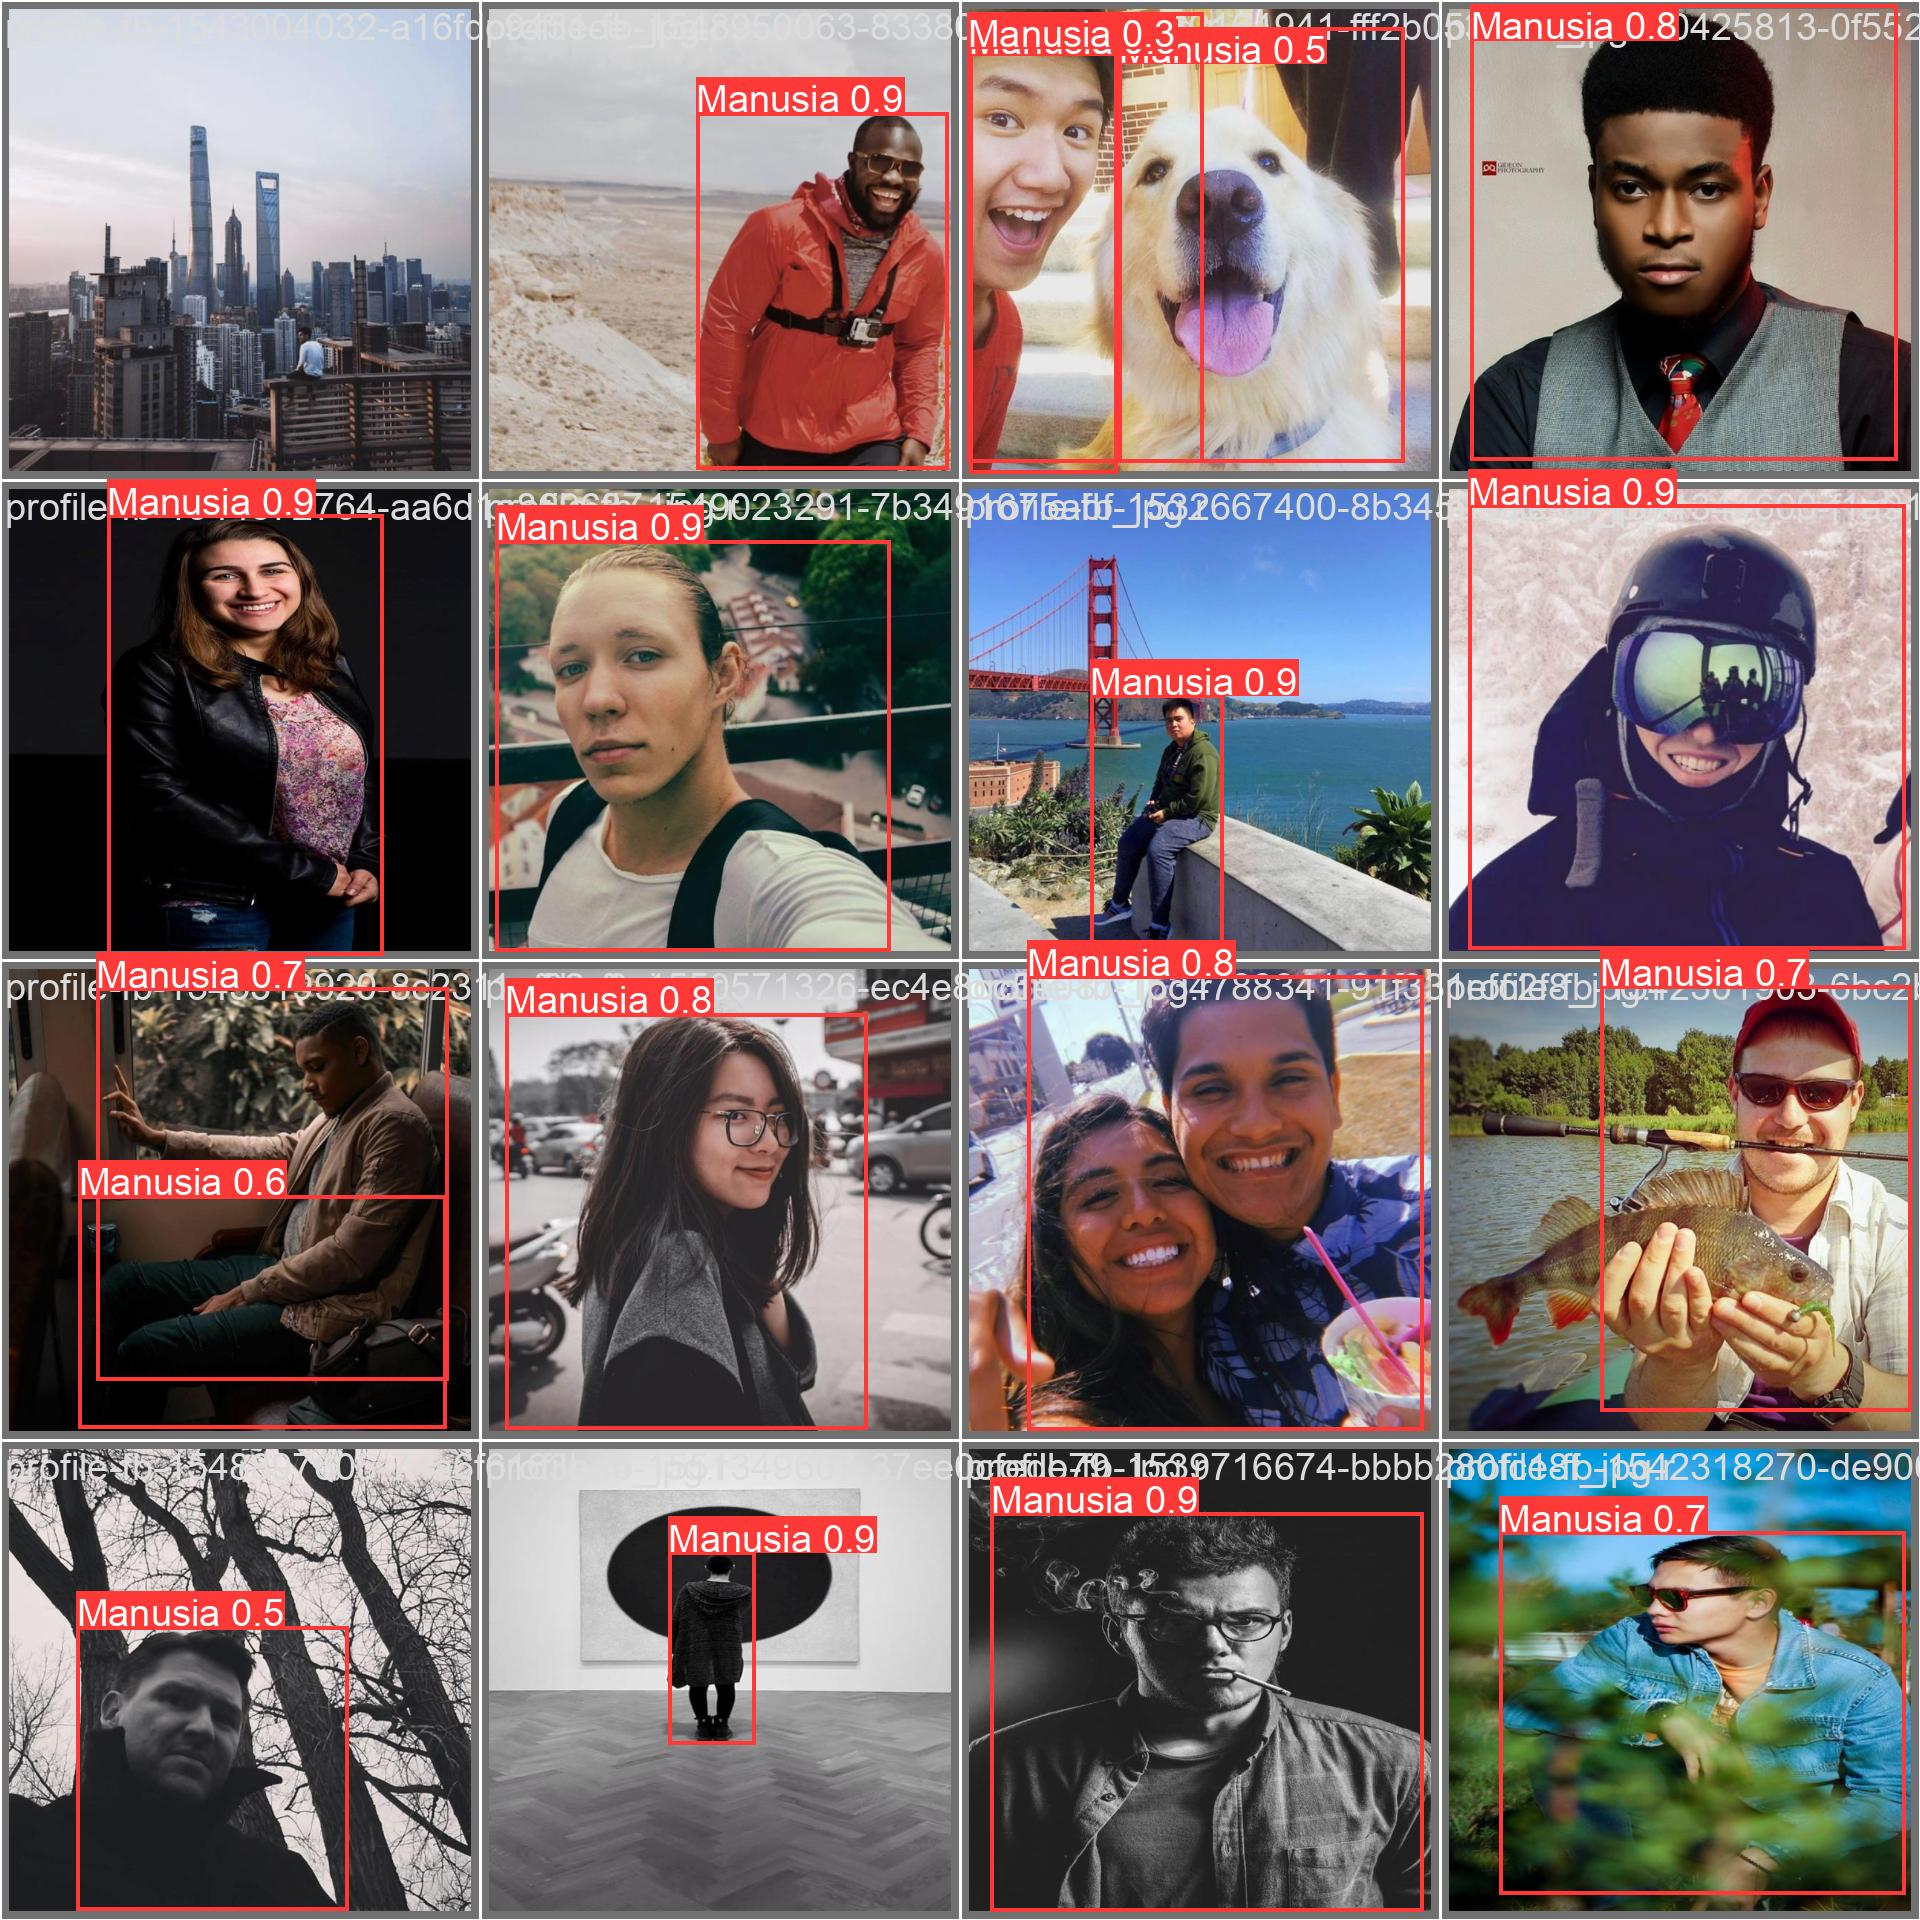
\includegraphics[scale=0.1]{gambar/confiden 150 epoch.jpg}
    \caption{Tes Inferensi Menggunakan Model Terlatih}
    \label{fig:visualisasi hasil training}
\end{figure}

\begin{figure}[H]
    \centering
    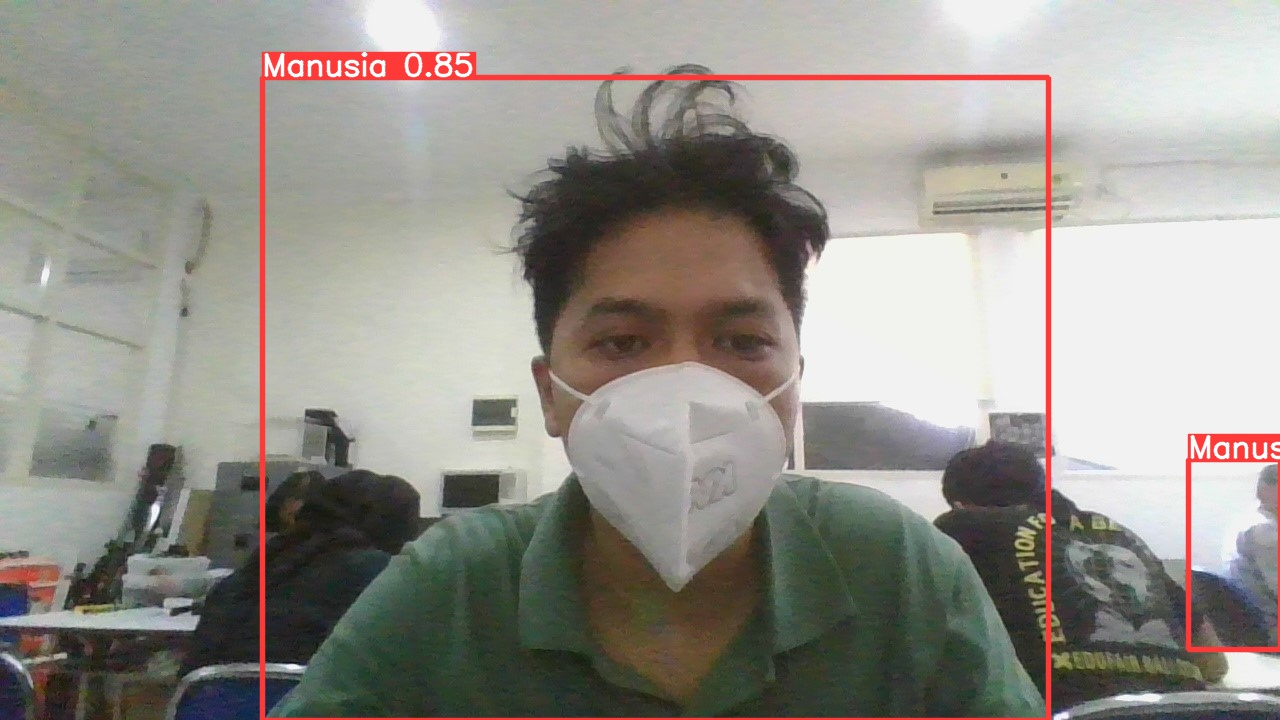
\includegraphics[scale=0.2]{gambar/confiden foto agung 150 epoch.jpg}
    \caption{Tes Inferensi Menggunakan Model Terlatih}
    \label{fig:enter-label}
\end{figure}

\subsubsection*{Perbandingan Evaluasi}

Dari kedua hasil training tersebut akan diambil yang terbaik berdasarkan pertimbangan akurasi. Dimana hasil dari confusion matrix kedua training menunjukan hasil yang baik, untuk lebih memahami kemampuan dari model maka perlu dihitung menggunakan rumus evaluasi sebagai berikut :

\begin{equation}
    Accuracy = \frac{TP + TN}{TP + TN + FP + FN}
\end{equation}

Sehingga dengan menginput masing nilai confusion matrix sebagai berikut :

\begin{lstlisting}[language=Python]
# Asumsi FP dan TN 0 Karena tidak ada nilai prediksi lain kecuali kelas manusia
TP_100 = 1806
FN_100 = 483
TP_150 = 1800
FN_150 = 489
FP_150_assumed = 0
FP_100_assumed = 0

accuracy_150_assumed = TP_150 / (TP_150 + FN_150 + FP_150_assumed)
accuracy_100_assumed = TP_100 / (TP_100 + FN_100 + FP_100_assumed)

accuracy_150_assumed, accuracy_100_assumed
\end{lstlisting}

Dari hasil perhitungan diatas didapatkan nilai akurasi untuk masing training dengan epoch 100 dan 150 yaitu sebesar 78.90\% dan 78.64\%. Dari 2 nilai tersebut didapatkan indikasi bahwa mengurangi jumlah epoch tidak berpengaruh signifikan terhadap kemampuan model untuk mengenali manusia dengan benar, dan bahkan sedikit lebih efisien dalam hal ini. Ini bisa berguna untuk menghemat waktu dan sumber daya komputasi tanpa mengorbankan performa yang banyak. Sehingga dalam proses selanjutnya model dengan 100 epoch akan digunakan dalam melakukan pengujian pada NUC.




\section{Deployment Pada Hardware}
Proses Deployment yang dilakukan Pada bagian ini berupa evaluasi kinerja model yang diimplementasikan pada perangkat keras. Skenario untuk mengumpulkan data untuk pengujian dengan menggunakan kamera Logitech C920 yang dipasangkan pada kursi roda otonom untuk mendeteksi manusia. Pengujian kinerja deployment dilakukan terhadap model yang dihasilkan pada pelatahin dengan 100 epoch. Dimana implementasi ini untuk mengukur:
\begin{enumerate} 
    \item Performa FPS sistem deteksi pada NUC.
    \item Inference dan Response time pada sistem.
    \item Tingkat keberhasilan kursi roda otonom dalam menghindari manusia.
\end{enumerate}

\subsection{Performa Model Pada Intel NUC}
Berikut hasil deployment yang dilakukan pada Intel NUC. Instalasi model pada NUC menggunakan venv yang tersedia pada Visual Studio code ide. Instalasi library perlu dilakukan untuk menjalankan model pada Intel NUC. Model output model berupa perintah yang dikirimkan untuk menggerakan motor akan dicatat melalui perbandingan hasil pada terminal visual studio code dan pada Ardruino ide. Berikut merupakan contoh data mentah yang dihasilkan dari output deteksi : 

\begin{lstlisting}[language = python]
0: 480x800 1 Manusia, 102.8ms
Waktu respons MediaPipe: 0.03261 detik
FPS: 6.08
Manusia di kiri
Speed: 5.7ms preprocess, 102.8ms inference, 0.0ms postprocess per image at shape (1, 3, 480, 800)
Waktu respons YOLO: 0.000467 detik
\end{lstlisting}

Dapat dilihat nilai yang ditampilkan berupa Waktu response mediapipe, FPS dari sistem, posisi manusia , kecepatan preprocess, waktu inference pada sistem NUC, postprocess, dan waktu response YOLO.

Agar kita dapat dengan mudah membaca nilainya maka akan dilakukan proses olah data menggunakan python. Berikut merupakan teknik pengolahan data menjadi format CSV sebagai berikut:

\begin{lstlisting}[language = python]
import pandas as pd
import re

raw_data = """
0: 480x800 1 Manusia, 95.6ms
Waktu respons MediaPipe: 0.02218 detik
Jarak : 1.34
FPS: 6.37
Manusia di tengah
Speed: 5.2ms preprocess, 95.6ms inference, 0.0ms postprocess per image at shape (1, 3, 480, 800)
Waktu respons YOLO: 0.00047 detik
"""

def parse_data_block(block):
    lines = block.strip().split('\n')
    parsed_data = {
        'Inference': float(re.findall(r"(\d+\.\d+)ms", lines[0])[0]),
        'MediaPipe Response Time': float(re.findall(r"(\d+\.\d+) detik", lines[1])[0]),
        'Jarak': float(re.findall(r"Jarak : (\d+\.\d+)", lines[2])[0]),
        'FPS': float(re.findall(r"FPS: (\d+\.\d+)", lines[3])[0]),
        'Position': lines[4],
        'Preprocess Time': float(re.findall(r"(\d+\.\d+)ms preprocess", lines[5])[0]),
        'Postprocess Time': float(re.findall(r"(\d+\.\d+)ms postprocess", lines[5])[0]),
        'YOLO Response Time': float(re.findall(r"(\d+\.\d+) detik", lines[6])[0])
    }
    return parsed_data

blocks = raw_data.strip().split('\n\n')
data = [parse_data_block(block) for block in blocks]

df = pd.DataFrame(data)

csv_path = "/mnt/data/processed_data_v2.csv"
df.to_csv(csv_path, index=False)

csv_path, df.head()
\end{lstlisting}

Dengan menjalankan program tersebut akan didapatkan tabel yang berisikan Waktu response mediapipe, FPS dari sistem, posisi manusia , kecepatan preprocess, waktu inference pada sistem NUC, postprocess, dan waktu response YOLO. Nilai - nilai yang didapatkan dari program tersebut akan dilakukan pengujian pada bagian selanjutnya dan diambil kesimpulan.  

\subsection{Pengujian Berdasarkan FPS}
Pengujian FPS akan dilakukan pada dua device yang pertama adalah pengujian pada device Laptop, dan pengujian pada device NUC. Dalam pengujian ini akan diambil nilai FPS sesuai dengan output yang didapatkan dan sudah diolah pada bagian sebelumnya.

\subsubsection{1. Pengujian pada Laptop}
Pada pengujian ini akan diambil nilai FPS pada laptop. Spesifikasi laptop yang digunakan pada pengujian ini merupakan sebagai berikut :

\begin{longtable}{|c|c|}
  \caption{Spesifikasi Laptop}
  \label{tb:Spesifikasi Laptop}                                   \\
  \hline
  \rowcolor[HTML]{C0C0C0}
  \textbf{Komponen} & \textbf{Spesifikasi}  \\
  \hline
  CPU            & Intel(R) Core(TM) i5-10300H CPU @2.50GHz(8CPU)        \\
  RAM            & 16 GB DDR4-2666 SDRAM        \\
  GPU            & NVIDIA® GeForce RTX™ 2060 with Max-Q design           \\
  \hline
\end{longtable}
Dapat dilihat pada tabel dibawah, didapatkan pada pengujian ini nilai rata - rata FPS sebesar 13.140. Dimana nilai FPS tertinggi adalah sebesar 13.23 dan FPS paling rendah ialah 13.05. Kestabilan nilai pada Pengujian ini menandakan bahwa performa sistem yang dijalankan pada laptop berjalan dengan sangat baik dan efisien.
\begin{table}[H]
    \centering
    \caption{Tabel FPS pada Laptop}
    \label{tb:FPS pada Laptop}                          \\
    \begin{tabular}{|l|l|}
    \hline
        No & FPS \\ \hline
        1 & 13.23 \\ \hline
        2 & 13.23 \\ \hline
        3 & 13.23 \\ \hline
        4 & 13.23 \\ \hline
        5 & 13.23 \\ \hline
        6 & 13.23 \\ \hline
        7 & 13.23 \\ \hline
        8 & 13.23 \\ \hline
        9 & 13.23 \\ \hline
        10 & 13.23 \\ \hline
        11 & 13.23 \\ \hline
        12 & 13.23 \\ \hline
        13 & 13.23 \\ \hline
        14 & 13.23 \\ \hline
        15 & 13.05 \\ \hline
        16 & 13.05 \\ \hline
        17 & 13.05 \\ \hline
        18 & 13.05 \\ \hline
        19 & 13.05 \\ \hline
        20 & 13.05 \\ \hline
        21 & 13.05 \\ \hline
        22 & 13.05 \\ \hline
        23 & 13.05 \\ \hline
        24 & 13.05 \\ \hline
        25 & 13.05 \\ \hline
        26 & 13.05 \\ \hline
        27 & 13.05 \\ \hline
        28 & 13.05 \\ \hline
        29 & 13.05 \\ \hline
        30 & 13.05 \\ \hline
    \end{tabular}
\end{table} 

\subsubsection*{2. Pengujian pada NUC}
Pada pengujian ini akan diambil nilai FPS pada NUC. Spesifikasi NUC yang digunakan pada pengujian ini merupakan sebagai berikut :

\begin{longtable}{|c|c|}
    \caption{Spesifikasi NUC}
    \label{tb:Spesifikasi NUC}                             \\
    \hline   
    \rowcolor[HTML]{C0C0C0}
    \textbf{Komponen} & \textbf{Spesifikasi} \\
    \hline
  CPU            &  Intel® Core™ i7-1165G7        \\
  RAM            & 32 GBLPDDR4        \\
  OS            & Windows 11 Home Single Language           \\
\end{longtable}
Dapat dilihat pada tabel dibawah, didapatkan pada pengujian ini nilai rata - rata FPS sebesar 6.111. Dimana nilai FPS tertinggi yang didapatkan ialah 6.47 dan FPS paling rendah ialah 5.54. Performa yang dihasilkan pada NUC tergolong stabil namun hasilnya kurang mendekati performa laptop.

\begin{table}[H]
    \centering
    \caption{Tabel FPS pada NUC}
    \label{tb:TabelFPS}                                        \\
    \begin{tabular}{|l|l|}
    \hline
        No & FPS \\ \hline
        1 & 6.37 \\ \hline
        2 & 6.43 \\ \hline
        3 & 6.43 \\ \hline
        4 & 5.57 \\ \hline
        5 & 5.54 \\ \hline
        6 & 5.79 \\ \hline
        7 & 5.83 \\ \hline
        8 & 6.42 \\ \hline
        9 & 6.47 \\ \hline
        10 & 6.47 \\ \hline
        11 & 6.47 \\ \hline
        12 & 6.42 \\ \hline
        13 & 6.42 \\ \hline
        14 & 6.42 \\ \hline
        15 & 6.42 \\ \hline
        16 & 6.43 \\ \hline
        17 & 6.42 \\ \hline
        18 & 6.42 \\ \hline
        19 & 6.47 \\ \hline
        20 & 6.42 \\ \hline
        21 & 6.42 \\ \hline
        22 & 6.43 \\ \hline
        23 & 6.42 \\ \hline
        24 & 6.42 \\ \hline
        25 & 6.47 \\ \hline
        26 & 6.42 \\ \hline
        27 & 6.42 \\ \hline
        28 & 6.37 \\ \hline
        29 & 6.43 \\ \hline
        30 & 6.33 \\ \hline
    \end{tabular}
\end{table}
 
\subsection{Pengujian Berdasarkan Hasil Response Time}
Untuk dapat melakukan pengujian hasil response time, maka obstacle harus memenuhi syarat Near Object Condition yang telah dibahas pada bab sebelumnya. Output yang dihasilkan setiap kali penghindaran berisi Arah dan time stamp pada Ardruino IDE dan Visual Studio code. Berikut merupakan contoh data mentah untuk kedua hasil output: 

\begin{lstlisting}[language=c]
22:18:32.273 -> Stop
22:18:32.948 -> Arah : E
22:18:33.131 -> Kanan
22:18:33.759 -> Arah : C
22:18:33.936 -> Stop
22:18:34.748 -> Arah : B
22:18:35.121 -> Maju
22:18:35.439 -> Arah : C
22:18:35.815 -> Stop
22:18:36.410 -> Arah : E
22:18:36.616 -> Kanan
\end{lstlisting}


Output yang didapatkan pada ardruino berisikan Timestamp. Timestamp yang dihasilkan yaitu \emph{Timestamp Receive ESP} dan \emph{Timestamp Receive Motor}. Selain pada ardruino pada vscode juga didapatkan nilai time stamp \emph{sent}, contoh outputnya dapat dilihat sebagai berikut.

\begin{lstlisting}[language=python]
BELOK KANAN,0.8,2024-05-08 22:18:14.263
MAJU,0.4,2024-05-08 22:18:18.762
BELOK KANAN,0.0,2024-05-08 22:18:28.614
MAJU,0.0,2024-05-08 22:18:30.940
BELOK KANAN,1.2,2024-05-08 22:18:32.899
MAJU,0.8,2024-05-08 22:18:34.728
BELOK KANAN,0.0,2024-05-08 22:18:36.392
\end{lstlisting}

Berdasarkan output diatas dapat dihitung Response Time sistem yang akan jabarkan pada tabel selanjutnya Hasil Response Time akan diuji untuk mendapatkan waktu yang dibutuhkan untuk melakukan pendeteksian dengan model yang kemudian diklasifikasi dan dikirim ke ESP32 hingga mo tor kursi roda mulai bergerak. Pengujian ini dilakukan secara real time pada perangkat NUC, perhitungan delay didapatkan dari mulai dikirim hingga berhentinya motor pada kursi roda. sedangkan perhitungan inference time dimulai dari dimulainya proses prediksi hingga didapatkan hasil dari proses klasifikasi. Rata - rata waktu delay yang didapatkan adalah 0.248 dari data yang sudah didapatkan dari pengujian NUC, adapun hasil nya dapat dilihat pada tabel dibawah. Adapun nilai inference rata-rata yang didapatkan adalah 
\begin{table}[H]
    \caption{Hasil Pengujian Response Time}
    \centering
    \begin{tabular}{|l|l|l|l|l|l|}
    \hline
        Inference & Sent & Receive & Motor & Delay & Arah \\ \hline
        125.0 & 19:53:02.763 & 19:53:02.800 & 19:53:03.178 & 0.378 & Stop \\ \hline
        131.5 & 19:53:06.543 & 19:53:06.572 & 19:53:06.760 & 0.188 & Maju \\ \hline
        139.5 & 19:53:08.800 & 19:53:08.826 & 19:53:09.014 & 0.188 & Stop \\ \hline
        154.1 & 19:53:14.058 & 19:53:14.118 & 19:53:14.450 & 0.262 & Kanan \\ \hline
        131.6 & 19:53:17.932 & 19:53:17.974 & 19:53:18.162 & 0.188 & Stop \\ \hline
        141.9 & 19:53:19.645 & 19:53:19.667 & 19:53:19.855 & 0.188 & Kiri \\ \hline
        136.7 & 19:53:29.266 & 19:53:29.287 & 19:53:29.477 & 0.190 & Stop \\ \hline
        132.7 & 19:53:35.816 & 19:53:35.854 & 19:53:36.230 & 0.376 & Maju \\ \hline
        152.5 & 19:53:42.816 & 19:53:42.868 & 19:53:43.059 & 0.191 & Stop \\ \hline
        136.5 & 19:53:46.210 & 19:53:46.249 & 19:53:46.437 & 0.188 & Kiri \\ \hline
        141.8 & 19:53:55.093 & 19:53:55.124 & 19:53:55.314 & 0.190 & Stop \\ \hline
        140.1 & 19:54:01.549 & 19:54:01.586 & 19:54:01.766 & 0.180 & Kanan \\ \hline
        127.5 & 19:54:03.265 & 19:54:03.319 & 19:54:03.509 & 0.190 & Stop \\ \hline
        135.5 & 19:54:04.964 & 19:54:05.010 & 19:54:05.373 & 0.363 & Kiri \\ \hline
        142.5 & 19:54:20.862 & 19:54:20.886 & 19:54:21.073 & 0.187 & Stop \\ \hline
        136.6 & 19:54:22.398 & 19:54:22.440 & 19:54:22.819 & 0.379 & Maju \\ \hline
        123.1 & 19:54:24.094 & 19:54:24.133 & 19:54:24.323 & 0.190 & Stop \\ \hline
        143.4 & 19:54:32.486 & 19:54:32.517 & 19:54:32.713 & 0.196 & Kiri \\ \hline
        141.6 & 19:54:34.426 & 19:54:34.492 & 19:54:34.871 & 0.379 & Stop \\ \hline
        129.6 & 19:54:36.177 & 19:54:36.231 & 19:54:36.376 & 0.145 & Kanan \\ \hline
        152.1 & 19:54:37.870 & 19:54:37.923 & 19:54:38.111 & 0.188 & Stop \\ \hline
        134.2 & 19:54:40.144 & 19:54:40.177 & 19:54:40.546 & 0.369 & Kiri \\ \hline
        136.4 & 19:54:42.220 & 19:54:42.234 & 19:54:42.422 & 0.188 & Stop \\ \hline
        133.5 & 19:54:43.909 & 19:54:43.926 & 19:54:44.289 & 0.363 & Kanan \\ \hline
        137.1 & 19:54:51.301 & 19:54:51.333 & 19:54:51.523 & 0.190 & Stop \\ \hline
        140.1 & 19:54:54.763 & 19:54:54.796 & 19:54:55.142 & 0.346 & Kiri \\ \hline
        135.5 & 19:54:56.502 & 19:54:56.551 & 19:54:56.742 & 0.191 & Stop \\ \hline
        181.1 & 19:54:58.584 & 19:54:58.619 & 19:54:58.981 & 0.362 & Maju \\ \hline
        141.5 & 19:55:00.444 & 19:55:00.487 & 19:55:00.678 & 0.191 & Stop \\ \hline
        149.5 & 19:55:05.502 & 19:55:05.576 & 19:55:05.936 & 0.360 & Kanan \\ \hline
    \end{tabular}
\end{table}

\subsection{Performa Keberhasilan}
Pengujian ini dilakukan pengetesan terhadap kursi roda dalam menghindari Manusia secara real time. Pengetesan ini akan dilakukan Pada Tower 2 ITS. Pada pengujian ini diambil 20 kali sampel dan dicatat keberhasilan penghindaran. Manusia yang dideteksi Diam dan tidak bergerak. Hasil yang didapatkan sebagai berikut 

\begin{table}[H]
\centering
\begin{tabular}{|l|l|}
\hline
Percobaan Ke & Hasil                                                               \\ \hline
1            & \cellcolor[HTML]{67FD9A}Kursi Roda Berhasil Menghindar              \\ \hline
2            & \cellcolor[HTML]{67FD9A}Kursi Roda Berhasil Menghindar              \\ \hline
3            & \cellcolor[HTML]{67FD9A}Kursi Roda Berhasil Menghindar              \\ \hline
4            & \cellcolor[HTML]{67FD9A}Kursi Roda Berhasil Menghindar              \\ \hline
5            & \cellcolor[HTML]{67FD9A}Kursi Roda Berhasil Menghindar              \\ \hline
6            & \cellcolor[HTML]{67FD9A}Kursi Roda Berhasil Menghindar              \\ \hline
7            & \cellcolor[HTML]{67FD9A}Kursi Roda Berhasil Menghindar              \\ \hline
8            & \cellcolor[HTML]{67FD9A}Kursi Roda Berhasil Menghindar              \\ \hline
9            & \cellcolor[HTML]{67FD9A}Kursi Roda Berhasil Menghindar              \\ \hline
10           & \cellcolor[HTML]{67FD9A}Kursi Roda Berhasil Menghindar              \\ \hline
11           & \cellcolor[HTML]{FD6864}Objek tidak terdeteksi dan Gagal Menghindar \\ \hline
12           & \cellcolor[HTML]{67FD9A}Kursi Roda Berhasil Menghindar              \\ \hline
13           & \cellcolor[HTML]{67FD9A}Kursi Roda Berhasil Menghindar              \\ \hline
14           & \cellcolor[HTML]{67FD9A}Kursi Roda Berhasil Menghindar              \\ \hline
15           & \cellcolor[HTML]{67FD9A}Kursi Roda Berhasil Menghindar              \\ \hline
16           & \cellcolor[HTML]{67FD9A}Kursi Roda Berhasil Menghindar              \\ \hline
17           & \cellcolor[HTML]{67FD9A}Kursi Roda Berhasil Menghindar              \\ \hline
18           & \cellcolor[HTML]{67FD9A}Kursi Roda Berhasil Menghindar              \\ \hline
19           & \cellcolor[HTML]{67FD9A}Kursi Roda Berhasil Menghindar              \\ \hline
20           & \cellcolor[HTML]{67FD9A}Kursi Roda Berhasil Menghindar              \\ \hline
\end{tabular}
\end{table}

Berdasarkan Hasil yang didapatkan Penghindaran berhasil sebanyak 19 kali dan gagal 1 kali pada percobaan ke 11. Adapun presentasi yang didapatkan dari hasil uji ini sebesar 98\%